% ========== KORTNÆBBET GÅS ==========
\begin{frame}{%
  \begin{minipage}[c]{0.30\textwidth}
    Kortnæbbet gås
  \end{minipage}%
  \hfill
  \begin{minipage}[c]{0.45\textwidth}
    \footnotesize
    \textbf{Jagttid:} 1.\ september -- 31.\ januar
  \end{minipage}%
  \hfill
  \begin{minipage}[c]{0.15\textwidth}
    \noindent\raggedleft
    
\includegraphics[width=0.5cm, height=0.5cm, keepaspectratio]{Billeder/Ikoner/star.png}%
    \hspace{0.2em}%
    
\includegraphics[width=0.5cm, height=0.5cm, keepaspectratio]{Billeder/Ikoner/star.png}
  \end{minipage}%
}
  \vspace{0.25em}
  \begin{columns}[T]
    % --- Venstre kolonne: Tekst ---
    \column{0.45\textwidth}
    \setlength{\parskip}{0.5em}
    \tiny
    \RaggedRight
    \textbf{\textit{Anser brachyrhynchus}} – kendes på det korte næb, men forveksles let med de øvrige grå gæs \par
    \textbf{Udseende:}\\
    \quad – Kort kraftigt lyserødt næb, lyserøde ben \par
    \textbf{Levesteder:} Vådområder og landbrugsarealer. \par
    \textbf{Føde:} Planteføde. \par
    \textbf{Udbredelse:} Langs vestkysten som trækfugl. \par
    \textbf{Træk/standfugl:} Trækfugl
    % --- Højre kolonne: Større billede ---
    \column{0.52\textwidth}
    \centering
    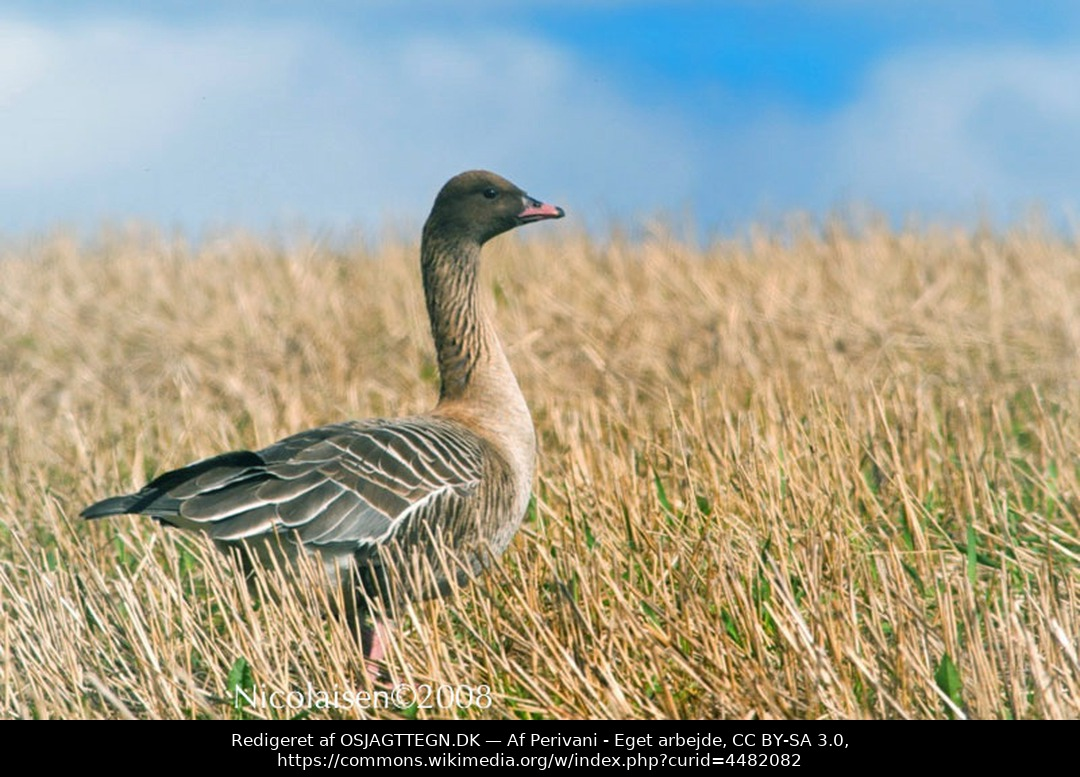
\includegraphics[width=\linewidth, height=7.2cm, keepaspectratio]{Billeder/Dyr/Fugle/Gaes/kortnæbbet_gås.jpg}
  \end{columns}
\end{frame}